\section{FIVE Web Framework}\label{framework}

FIVE, acronym of \emph{Framework for Indoor mapping in Virtual Environments},
provides a customizable, and scalable web framework realizing an virtual
indoor mapping platform in which multiple applications can convenient resides
on at the same time: IoT monitoring, realtime multi-person tracking and
cross-storey user navigation.

Expandability and customizability derive from both design choices and
HIJSON format inherent characteristics, i.e.~the possibility of semantic extensions (see Section~\ref{semantic-extensions}).
Scalability is directly borrowed from technologies used for
software development: \emph{JavaScript} language, using \emph{Node.js},
in particular \emph{Express.js} as backend framework, exploiting the
power of WebSocket protocol through the \emph{Socket.io} library.

Being supported by the \emph{web-as-a-platform}, the framework exposes
also an high availability: it is so simple to use as to visit a
website, both from desktop or mobile devices, without explicit
requirements to install any software package from proprietary stores---access to
which is often denied from business devices.

The FIVE Web Framework deeply relies on HIJSON Toolkit (see Section~\ref{toolkit}) and offers an
all-inclusive client/server architecture with a convenient and highly interactive
user interface, leaving aside the specific indoor positioning system and
the IoT sensors to deal with. A robust application interface is provided and
described in the following section.

\subsection{Applications}\label{applications}

The Framework has been designed with focus on two different kind of
users: the \emph{Explorer} and the \emph{Supervisor}. They have
different requirements and are likely equipped with different devices:
while the \emph{Supervisor} monitors the indoor environment through a
desktop workstation, the \emph{Explorer} has a smartphone available and
needs to be routed across the building.

In both cases, the web platform ensures a perfect alignment with the
BYOD (Bring Your Own Device) approach, nowadays often supported by companies
that encourage employees to use personal devices.


\subsubsection{IoT monitoring}\label{iot-monitoring}

An \emph{IoT monitoring application} consists of an interface showing to the
user, in a single, integrated and centralized way, the information collected
from all the smart objects modelled in the HIJSON document. IoT monitoring
application provides bidirectional communication, since the interface let the
user receive information coming from smart objects while allowing him to send
commands to them.

As the name itself may suggest, it is an activity specifically performed by a
\emph{Supervisor} user, but it can be also suitable to be deployed for the
\emph{Explorer} user, since she can take advantage of the interactive
information coming from the surroundings objects while she moves across the
indoor environment.

Monitoring different smart objects may require different ways to visualize
and/or send data and commands. Modularity and extendibility of the application
respond superbly to these requirements, by providing for each class of objects
a different interface of visualization and interaction, as a result of the
polymorphism principles introduced by the HIJSON Class. In particular, the
user interface is characterized by a dual-display mode, that allows the user
to see at the same time a 2D map that gives an overall glance in a simplified
plan, and a 3D virtual environment to navigate into, as shown in
Figure~\ref{fig:web-framework-ui}.

Alongside with typical smart objects, suitable to deal with like thermostats,
where the user can read the room  temperature and turn the heating on/off,
other kinds of objects, that are not properly considered ``smart'', can be
integrated into the FIVE environment. It is the case, for example, of fire
extinguishers, that are able to show the date of their last check, stored in a
database.

\subsubsection{Realtime multi-person tracking}\label{realtime-multi-person-tracking}

Realtime multi-person tracking allows a \emph{Supervisor} to monitor the
actual position of people inside the building. This kind of task can be useful
for several reasons, including security, logistics or to supervise composite
operative workflows. Each device equipped with the \emph{Explorer} application
is in charge of locating itself, interacting with the indoor positioning
system, and notifying the current position in continuos mode. Evidence of the
people position is given to the \emph{Supervisor} both into a 2D map and an
immersive 3D virtual environment (see Figure~\ref{fig:web-framework-ui}).

\subsubsection{Cross-storey user navigation}\label{cross-storey-user-navigation}

The FIVE Framework also provides the capability to give directions to
\emph{Explorer} users that must move across the indoor environment. The user
specifies a starting and an ending point and the system provides him with a
valid connection path. This feature strongly rely on the graph of paths
generated by the Toolkit (see Section~\ref{automatic-generation-of-valid-paths}), so
starting and ending points must be nodes of the graph. \emph{Connection nodes}
are introduced to represent stairs or elevators, enabling cross-storey paths
to be computed. Since paths can span more than one storey, the most effective
way to display them to the user is to show the connection nodes visualized in
one or more 2D maps.

\subsection{Architecture}\label{architecture}

\begin{figure*}[htb]
\centering
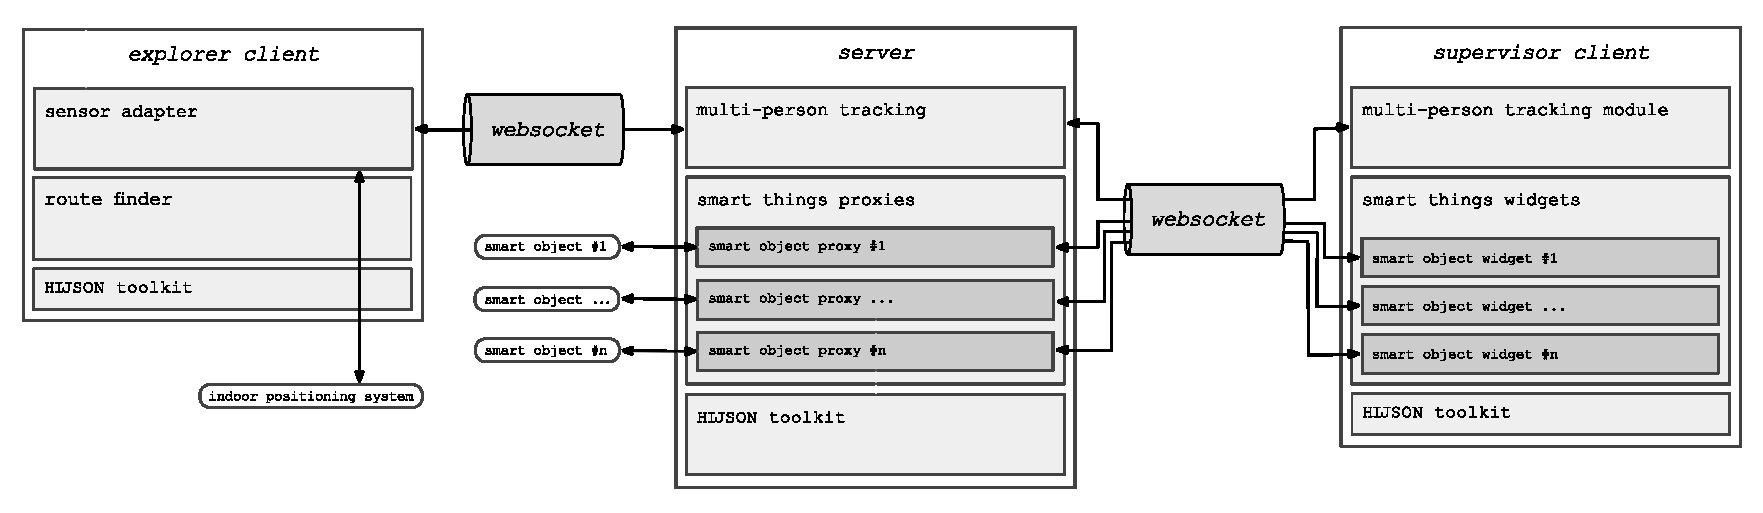
\epsfig{file=images/architecture.eps, width=\textwidth}
\caption{FIVE Web Framework architecture}
\label{fig:architecture}
\end{figure*}

Like the vast majority of the web based applications, the Framework exposes an
overall architecture that is inherently \emph{client/server}. In particular,
two different types of possible clients are identifiable, one for each different 
kind of users: the \emph{Supervisor} client and the \emph{Explorer} client. 
Both of them connect to the same server.

The indoor space described by the input HIJSON document is processed by the
server via the processing pipeline (see Section~\ref{pipeline}). After that, any
connecting \emph{Explorer} client, presumably via a mobile device, will be
provided with the information to perform cross-storey navigation of the
building, while reporting the user position to the server. The server will
feed any connecting \emph{Supervisor} client with users positions, along with
data from sensor-equipped  objects present in the environment, achieving both
IoT monitoring and realtime multi-person tracking.

\subsubsection{Server Architecture}\label{server-architecture}

An architectural scheme of the framework is provided in
Figure~\ref{fig:architecture}. A web server module is responsible for
listening to connecting clients. Each client connection is handled by the web
server module providing all the required resources and then by opening a
WebSocket channel, in order to have both \emph{Explorer} and/or
\emph{Supervisor} communication protocol data flow within. In particular, the
\texttt{multi-person\ tracking} module receives position data from
\emph{Explorer} clients. It aggregates and sends these information to
connected \emph{Supervisor} clients through the WebSocket channel, using a
simple but reliable protocol described later. Independence from particular IoT
sensor equipment communication protocols is achieved introducing a
\texttt{smart\ object\ proxy} module. This one is defined in the HIJSON Class
and is obtained via the \texttt{getProxy()} method (see Section~\ref{hijson-class-definition}) 
for each smart object modelled as described in the follow.

\subsubsection{Explorer client architecture}\label{explorer-client-architecture}

The \emph{Explorer} client architecture is generally deployed on a mobile
device, which is usually supplied to a user who needs to be routed across the indoor mapped
environment. The \texttt{sensor\ adapter} module
encapsulates the communication logic with the indoor positioning system. The
presence of this module ensures independence from particular technologies, so
allowing the \emph{Explorer} client to rely on different indoor positioning
systems (Wi-Fi, Bluetooth, LTE, etc.).

Every time a \texttt{sensor\ adapter} observes a perceptible modification in
user position, it sends the new position information to the server through the
single opened WebSocket, spawning a simple message which includes, beside
current coordinates, the information of the storey of the possibly multilevel
building the user is in.

It is to remark that, when not outflanked by the introduction of an external
server, the problem of communication between positioning system and the low
level APIs of the browser is left to positioning system itself or to whom is
in charge of specific deployments of the FIVE Web Framework.
The \texttt{smart\ object\ widget} module, being in common with the
 \emph{Supervisor} client, will be discussed in the next section.

\subsubsection{Supervisor client architecture}\label{supervisor-client-architecture}

The architecture of \emph{Supervisor} client includes two modules. The first
one, named \texttt{multi-person\ tracking} module, is responsible to
receive through the WebSocket, from the server information about
\emph{explorers} of the environment, showing them in the user interface. The
second module, named \texttt{smart\ object\ widget}, communicates with the
server to propose the user realtime information about sensor-equip\-ped
objects in the environment. Data passes through the single WebSocket
opened between the server and every \emph{Supervisor} client. Relying on a
naive but effective communication protocol, each \texttt{smart object widget}
exchanges data only with its corresponding \texttt{smart object proxy} on the server. To
ensure the data are posted only when the user requires the information
relative to a specific smart object, a \emph{widget lifecycle protocol} is
implemented. This one is based on the four event triggers \texttt{on\_before\_show},
\texttt{on\_show}, \texttt{on\_before\_hide}, \texttt{on\_hide}, as suggested by their names.
When the user requires information about a smart object, its widget has
to be rendered, and \texttt{on\_before\_show} the server is notified to
connect via relative proxy to the sensor. Once connected, the server
begin to send data via WebSocket. Received data are shown through the
widget to the user. When done, the \texttt{on\_before\_hide} event of the
widget is triggered, a notification is sent to the server announcing to stop sending
data, and the proxy closes the connection to the sensor. Widget lifecycle
protocol ensures that only required data are sent from the server to the
client.
